\documentclass[a4paper,12pt]{article}
\usepackage[utf8]{inputenc}
\usepackage[vietnamese]{babel}
\usepackage{hyperref}
\usepackage{xcolor}
\usepackage{graphicx}
\usepackage{caption}

% Set margin adjustments if necessary
\usepackage[a4paper, margin=1in]{geometry}

\title{\textbf{Dự án Chuỗi cung ứng sử dụng Hyperledger Fabric và React}}
\date{19/3/2025}

\begin{document}
\maketitle
\begin{center}
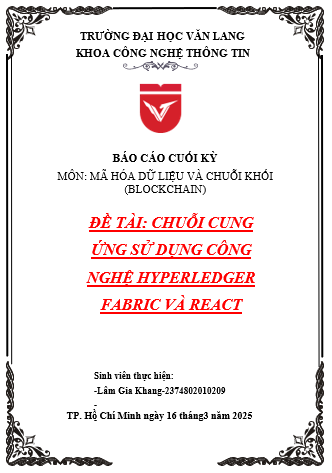
\includegraphics[scale=2]{Anh/A1.png}
\end{center}
{\color{red} \section{Giới thiệu cơ bản}}
{\color{red} \subsection{Tổng quan về Blockchain}}
+ Blockchain là một hệ thống lưu trữ và truyền tải thông tin các giá trị giao dịch theo mô hình ngang hàng (peer-to-peer) dựa trên các khối liên kết với nhau, thông qua mã hoá tạo thành một chuỗi các khối.\\
\textbf{- Cấu trúc của dữ liệu khối blockchain:}
\begin{center}
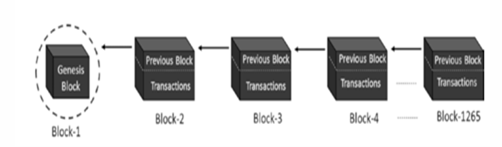
\includegraphics[scale=1.2]{Anh/A2.png}
\end{center}
\begin{itemize}
- \textbf{Genesis Block}: Khối đầu tiên trong chuỗi blockchain\\
- \textbf{Previous Block}: Khối ngay trước khối hiện tại trong chuỗi blockchain\\
- \textbf{Transactions}: Là các giao dịch được ghi lại trong blockchain, bao gồm các thông tin\\
\textbf{+ Quy trình hoạt động:}
\end{itemize}
\begin{center}
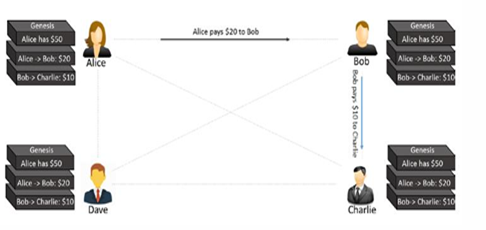
\includegraphics[scale=1.5]{Anh/A3.png}
\end{center}\vspace{10cm}
\textbf{+ Lợi ích của blockchain:}\\
- Không thể làm giả, không thể phá hủy các chuỗi blockchain:\\
- Bất biến\\
- Bảo mật Dữ liệu\\
- Minh bạch\\
- Hợp đồng thông minh\\
\textbf{+ Các ứng dụng của blockchain:}\\
- Tiền kỹ thuật số (Crypto currency)\\
- Quản lý chuỗi cung ứng (Supply chain)\\
- Y tế\\
- Giáo dục\\

{\color{red} \subsection{Tổng quan về Hyperledger Fabric}}

+ Hyperledger Fabric là một loại permissioned blockchains (blockchain phân quyền có kiểm soát) giúp kiểm soát ai có quyền truy cập và thực hiện các hành động quan trọng nhằm tăng cường bảo mật và hiệu quả vận hành của mạng.

- Cấu trúc của mạng Hyperledger Fabric:
\begin{center}
- 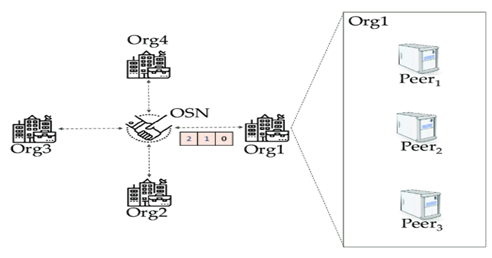
\includegraphics[scale=1.3]{Anh/A4.png}
\end{center}
\begin{itemize}
- \textbf{Org (organization)}: Là các thành viên của mạng Hyperledger Fabric, tương đương với 1 đại diện tham gia vào mạng lưới blockchain.\\
- \textbf{ONS (ordering node service)}: Một thành phần trong Hyperledger Fabric chịu trách nhiệm thu thập các giao dịch đã được xác nhận bởi các endorsing peer, sắp xếp theo thứ tự và đưa vào sổ cái.\\
- \textbf{Peer (nút mạng)}: Là một phần trong org, thực hiện lưu trữ bản sao của sổ cái (ledger) và thực thi các giao dịch (transactions) dựa trên các hợp đồng thông minh (chaincode).\\
\end{itemize}\vspace{5cm}
\textbf{+ Quy trình hoạt động:}
\begin{center}
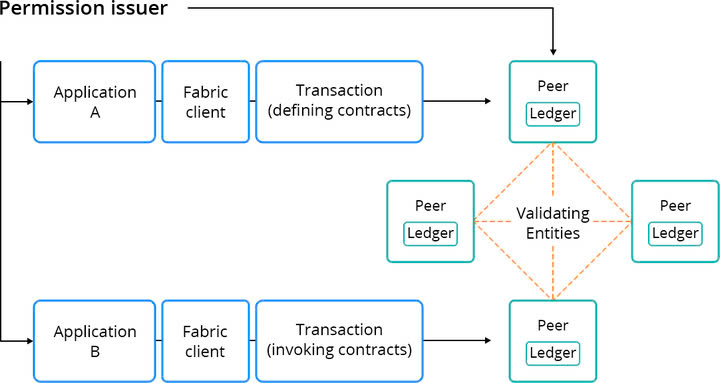
\includegraphics[scale=0.7]{Anh/A5.png}
\end{center}
\textbf{+ Lợi ích của Hyperledger Fabric:\\}
- Kiểm soát quyền truy cập\\
- Tăng cường bảo mật\\
- Hiệu quả vận hành của mạng\\
\textbf{+ Các ứng dụng của Hyperledger Fabric:\\}
- Quản lý chuỗi cung ứng (Supply chain)\\
- Theo dõi tài sản\\
- Các giải pháp doanh nghiệp phân quyền\\

{\color{red} \section{Dự án}}
{\color{red} \subsection{Thông tin cơ bản}}
+ Mục tiêu: Ứng dụng quản lý chuỗi cung ứng này được xây dựng trên nền tảng Hyperledger Fabric để cung cấp tính minh bạch và an toàn trong các giao dịch. Nó cho phép các bên tham gia chuỗi cung ứng như nhà sản xuất, nhà bán sỉ, nhà phân phối, nhà bán lẻ, và người tiêu dùng theo dõi và quản lý sản phẩm từ khâu sản xuất đến giao hàng cuối cùng.\\
\textbf{+ Đối tượng sử dụng}:
\begin{itemize}
- Nhà sản xuất\\
- Nhà bán sỉ/lẻ\\
- Nhà phân phối\\
- Người tiêu dùng\\
\end{itemize}

\textbf{+ Các trường hợp cần sử dụng}:
\begin{itemize}
- Theo dõi/truy xuất/xác minh/chứng thực nguồn gốc của thực phẩm từ trang trại đến bàn ăn\\
- Quản lý hàng hoá\\
- Chia sẻ thông tin của hàng hoá\\
\end{itemize}

{\color{red} \section{Ứng dụng}}
{\color{red} \subsection{Thông tin cơ bản}}

\textbf{+ Giới thiệu}: Dự án SupplyChain-HLF sử dụng Hyperledger Fabric (HLF), một nền tảng blockchain mã nguồn mở nhằm quản lý chuỗi cung ứng,giúp giải quyết các vấn đề:
\begin{itemize}
- Theo dõi sản phẩm trong toàn bộ chuỗi cung ứng\\
- Chia sẻ chuỗi cung ứng cho các bên tham gia\\
- Xác minh và chứng thực sản phẩm trong chuỗi\\
- Cung cấp khả năng kiểm toán tốt hơn\\
\end{itemize}
\textbf{+ Các chức năng của ứng dụng}:\\
- CreateUser (Admin): Tạo người dùng (Quản trị viên)\\
- SignIn (user Login): Đăng nhập (Đăng nhập người dùng)\\
- CreateProduct: (Manufacturer): Tạo sản phẩm (Nhà sản xuất)\\
- UpdateProduct (Manufacturer, Wholesaler, Distributor, Retailer): Cập nhật sản phẩm (Nhà sản xuất, Nhà bán buôn, Nhà phân phối, Nhà bán lẻ)\\
- SendToWholesaler: Gửi cho nhà bán buôn\\
- SendToDistributor: Gửi cho nhà phân phối\\
- SendToRetailer: Gửi cho nhà bán lẻ\\
- SellToConsumer: Bán cho người tiêu dùng\\
- QueryAsset (Query by Product ID): Truy vấn tài sản (Truy vấn theo ID sản phẩm)\\
- QueryAll (All): Truy vấn tất cả (Tất cả)\\
- OrderProduct1 (Consumer places order, productID -> Retailer): Đặt hàng sản phẩm (Người tiêu dùng đặt hàng, ID sản phẩm -> Nhà bán lẻ)   \\
- DeliveredProduct (Retailer Updates): Sản phẩm đã giao (Nhà bán lẻ cập nhật)\\
- Init : Khởi tạo - Khởi tạo bộ đếm về giá trị NIL (thường là 0 hoặc rỗng)\\
- Invoke chaincode: Gọi - Để gọi từng chức năng trong chaincode\\
\begin{itemize}

\end{itemize}

{\color{red} \subsection{Chi tiết}}

\textbf{+ Các thành phần của dự án}:
\begin{itemize}
- Ứng dụng giao diện người dùng bằng React.js\\
- API trung gian sử dụng Node.js\\
- Node.js SDK\\
- Mạng lưới – Hyperledger Fabric\\
- Chaincode - Golang\\
\end{itemize}

\textbf{Kiến trúc của ứng dụng}:\\
\textbf{a) Quy trình hoạt động}:
\begin{itemize}
- Bước 1: Người dùng đăng ký tài khoản qua một giao diện ứng dụng được phát triển bằng React.js, điền thông tin cá nhân và chi tiết vai trò.\\
- Bước 2: Quản trị viên yêu cầu cấp danh tính từ Certificate Authority (CA) để đăng ký danh tính cho người dùng mới.\\
- Bước 3: Quản trị viên cấp chứng chỉ cho người dùng thông qua CA.
- Bước 4: Cấp quyền và cấu hình vai trò người dùng bằng cách cập nhật quyền truy cập vai trò thông qua chaincode.\\
- Bước 5: Sau khi đăng ký hoàn tất, người dùng có thể sử dụng ứng dụng và thực hiện các thao tác tương ứng với vai trò.\\
\end{itemize}

\textbf{b) Quản lý quyền truy cập}:
\begin{itemize}
- Mỗi người dùng khi được đăng ký sẽ có một tập quyền riêng, quản trị viên sẽ đảm bảo rằng các quyền truy cập vào hệ thống được quản lý chính xác thông qua các chính sách truy cập (Access Control Policies).\\
- Chính sách này đảm bảo rằng người dùng chỉ có thể xem và thao tác với những dữ liệu mà họ được phép.\\
\end{itemize}

\textbf{c) Quản lý vòng đời sản phẩm}:
\begin{itemize}
- Sau khi người dùng được đăng ký, các nhà sản xuất sẽ có thể tạo sản phẩm mới và gửi chúng vào chuỗi cung ứng.\\
- Nhà sản xuất sử dụng ứng dụng để tương tác với blockchain và gửi các thông tin về sản phẩm (như mã sản phẩm, thông tin vận chuyển) lên blockchain.\\
\end{itemize}

\textbf{d) Quy trình theo dõi sản phẩm}:
\begin{itemize}
- Nhà bán sỉ, nhà phân phối, nhà bán lẻ sẽ nhận thông tin sản phẩm và thực hiện các giao dịch tương ứng khi sản phẩm được chuyển giao từ nhà sản xuất đến người tiêu dùng.\\
- Người tiêu dùng sau đó có thể đặt hàng và nhận sản phẩm, xác nhận qua ứng dụng rằng họ đã nhận hàng.\\
\end{itemize}

\textbf{e) Tổng quan luồng ứng dụng}:
\begin{itemize}
- Quản trị viên: Đăng ký người dùng vào hệ thống và cấp quyền truy cập.\\
- Nhà sản xuất: Tạo sản phẩm mới.\\
- Nhà bán sỉ, nhà phân phối, nhà bán lẻ: Nhận và gửi sản phẩm theo từng giai đoạn.\\
- Người tiêu dùng: Đặt hàng và xác nhận khi nhận sản phẩm.\\
\end{itemize}\vspace{10cm}
{\color{red} \section{Nguồn tham khảo/mã nguồn}}
\textbf{Nguồn tham khảo}:
\begin{itemize}
\url{https://github.com/huynhhoc/mahoa/blob/main/How%20To%20Install%20Hyperledger%20Fabric%20v2.4%20on%20Ubuntu%2020.04%20-%20DEV%20Community.pdf}
\url{https://www.investopedia.com/terms/b/blockchain.asp}
\url{https://www.geeksforgeeks.org/hyperledger-fabric-in-blockchain/}\\
\url{https://github.com/kuldeep23907/Supply-Chain-using-Hyperledger-Fabric-and-React}
\end{itemize}
\textbf{Mã nguồn app/hướng dẫn}: \\
{\color{red} \section{Kết luận}}
+ Tóm lại, dự án xây dựng ứng dụng quản lý chuỗi cung ứng sử dụng Hyperledger Fabric và React представляется một giải pháp đầy tiềm năng để giải quyết những thách thức hiện tại trong việc quản lý chuỗi cung ứng. Bằng cách tận dụng các ưu điểm của công nghệ blockchain về tính minh bạch, bảo mật và khả năng theo dõi, ứng dụng này có thể mang lại lợi ích đáng kể cho tất cả các bên tham gia, từ việc đảm bảo nguồn gốc sản phẩm đến việc nâng cao hiệu quả hoạt động và sự tin tưởng của người tiêu dùng.

\tableofcontents
\end{document}
